The signal extraction in the $WH\to WW^{*}$ channels yields an observed signal strength of 
$\mu = 0.82^{+0.45}_{-0.39}$, corresponding to an observed significance of approximately 2.3~$\sigma$, 
consistent with the Standard Model prediction. This measurement is dominated by the \zdep{} channel, 
which has an observed signal strength of $\mu = 1.16^{+0.59}_{-0.49}$ and an observed significance of 
about 2.7~$\sigma$, while the \zdom{} channel is found to have
$\mu = 0.40^{+0.81}_{-0.75}$ with an observed significance of roughly 0.5~$\sigma$. 
The opposite pulls from these two channels slightly reduce the combined significance relative to that 
of the \zdep{} channel alone. Both channels remain compatible with the Standard Model within uncertainties.

Compared to the previous Run~2 $WH \to WW^{*}$ analysis~\cite{ATLAS:2025abg}, the observed significance has increased from 1.8~$\sigma$ to 2.3~$\sigma$, reflecting the larger integrated luminosity of the Run~3 dataset, improvements in analysis techniques, and a higher $\mu$ value in the $\zdep{}$ channel, which is the primary driver of this result. In comparison to the CMS Run~2 analysis~\cite{CMS:2021ixs}, our measurement shows a lower observed significance despite a higher expected sensitivity. A key difference lies in the treatment of the 3$\ell$ channel: in this analysis, it is split into two signal regions, with a control region defined from one of them to constrain the $WWW$ background. This background exhibits a notable excess ($\mathrm{NF} = 1.84$), which is not accounted for in the CMS analysis and likely contributes to some of their sensitivity. It would be interesting to investigate whether a similar excess appears in the CMS dataset.

% In the STXS framework, the observed signal strengths in the combined \wh{} channel for the three $\ptv$ bins are found to be $\mu = 1.42^{+1.3}_{-1.1}$ for $\ptv < 75$~GeV, $\mu = 0.54^{+1.2}_{-1.0}$ for $75 \leq \ptv < 150$~GeV, and $\mu = 0.67^{+1.0}_{-0.8}$ for $\ptv \geq 150$~GeV. Compared to Run~2 our sensitivity is worse all around, but all of our POIs are in agreement with SM predictions. Our sensitivity probably suffers from a few things, but I will say that most of it stems from superior lepton isolation WPs and other important criteria that were available for Run~2 but are not yet there for Run~3. Comparing this analysis to the full Run~2 $VH(b\bar{b})$ analysis, shows the sensitivity that this channel has in the low \ptw{} bins. In Figure~\ref{fig:stxs_results_discussion}, the results from this analysis are compared to those from the Run~2 $VH(b\bar{b})$ analysis~\cite{ATLAS:2020gxx}. The $VH(b\bar{b})$ analysis doesn't bother measuring the lowest \ptv{} bin due to the overwhelming background contamination, resulting in no sensitivity. The $VH(b\bar{b})$ analysis also clearly struggles in the $75 \leq \ptv < 150$~GeV bin, where the measurement is consistent with zero and has a super large uncertainty. This is not the case for this analysis, which shows reasonable sensitivity in both of the lower \ptv{} bins. This highlights the importance of this channel in allowing us to probe the lower \ptv{} bins that are inaccessible to other analyses.
Within the STXS framework, the observed signal strengths in the combined \wh{} channel are measured to be $\mu = 1.42^{+1.3}_{-1.1}$ for $\ptv < 75$~GeV, $\mu = 0.54^{+1.2}_{-1.0}$ for $75 \leq \ptv < 150$~GeV, and $\mu = 0.67^{+1.0}_{-0.8}$ for $\ptv \geq 150$~GeV. Compared to Run~2, the overall sensitivity of this measurement is reduced; however, all POIs remain consistent with the Standard Model predictions. The reduced sensitivity is attributed primarily to limitations in lepton isolation working points and other selection criteria that were available during Run~2 but are not yet available for Run~3.

\begin{figure}[htp]
    \centering
    \subfloat[$WH(WW^{*})$ differential cross sections]{
        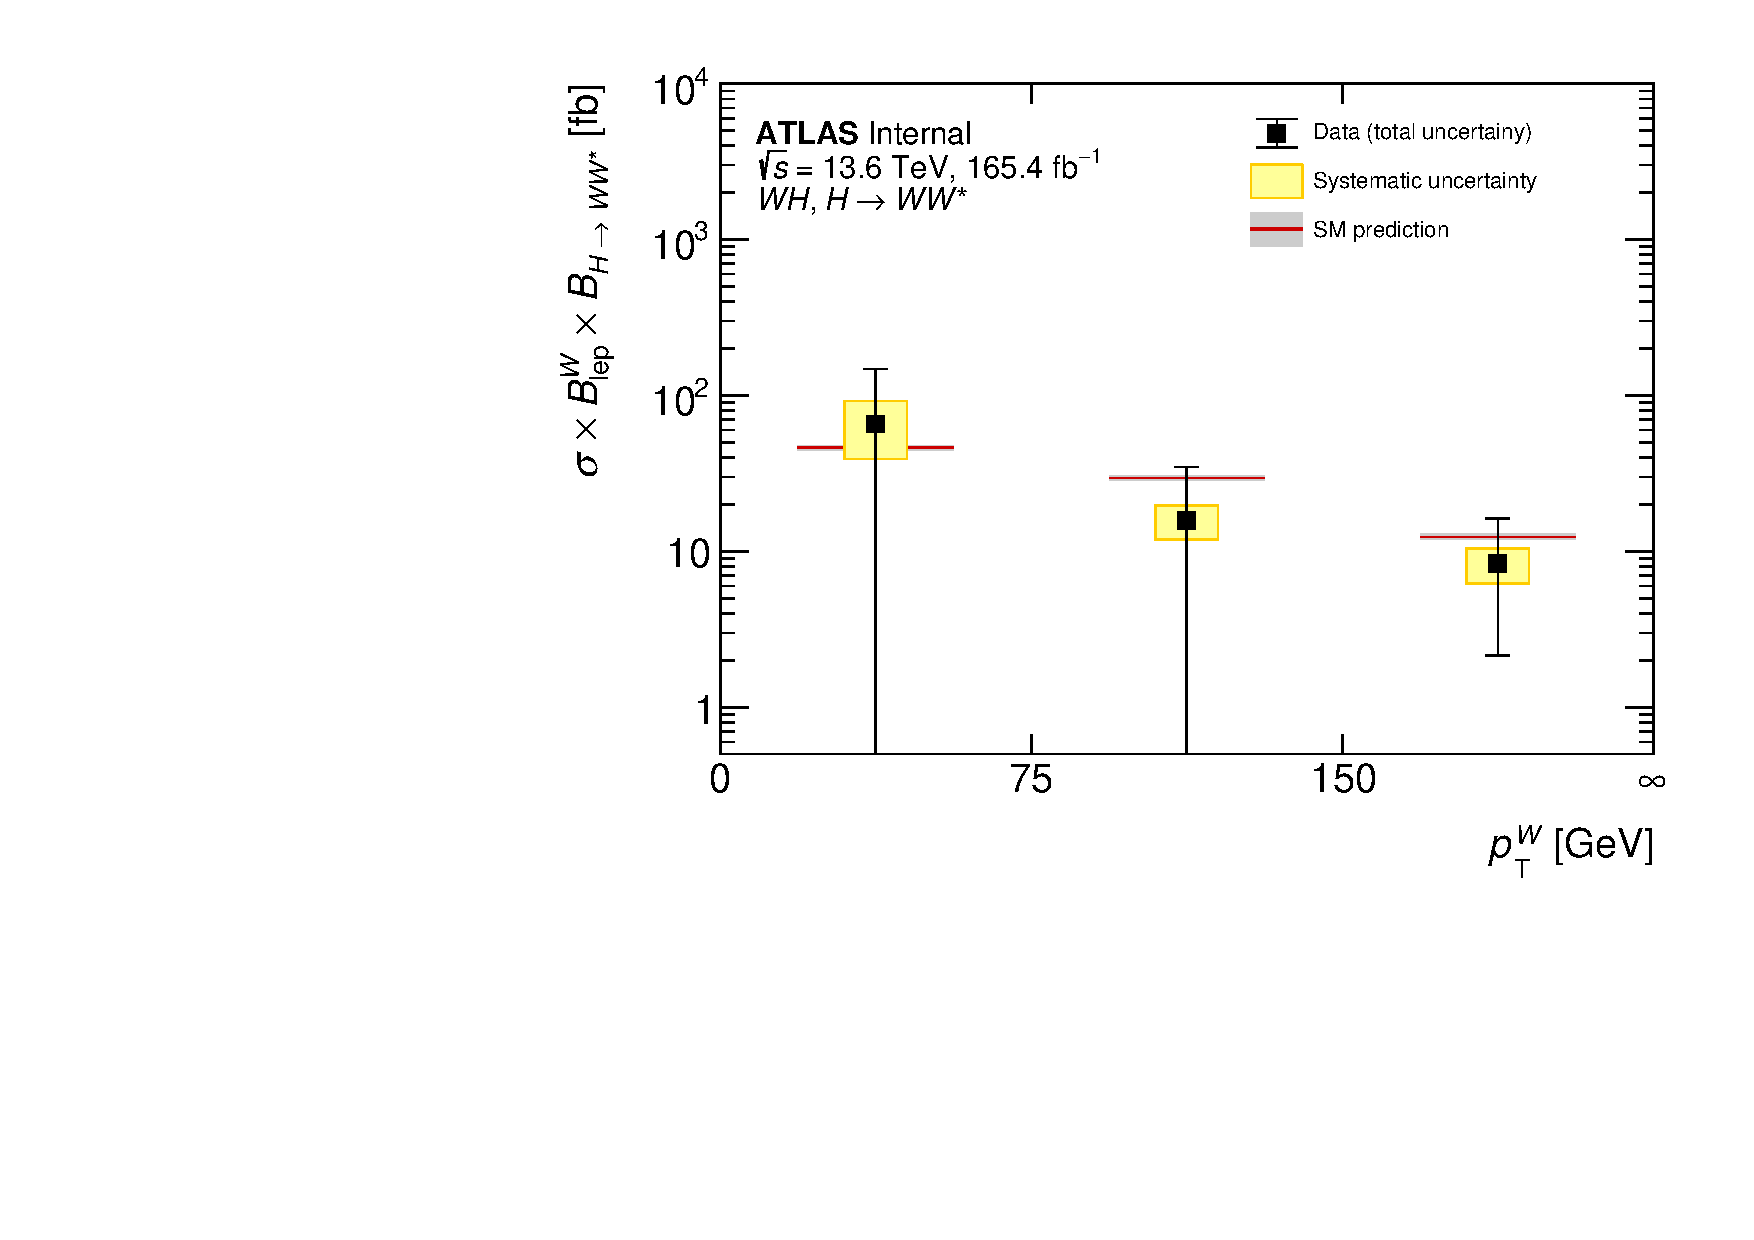
\includegraphics[width=0.45\textwidth]{figures/statistical/differential_cross_section.pdf}\label{fig:wh_stxs_results_plot}
    }
    \subfloat[$VH(b\bar{b})$ differential cross sections]{
        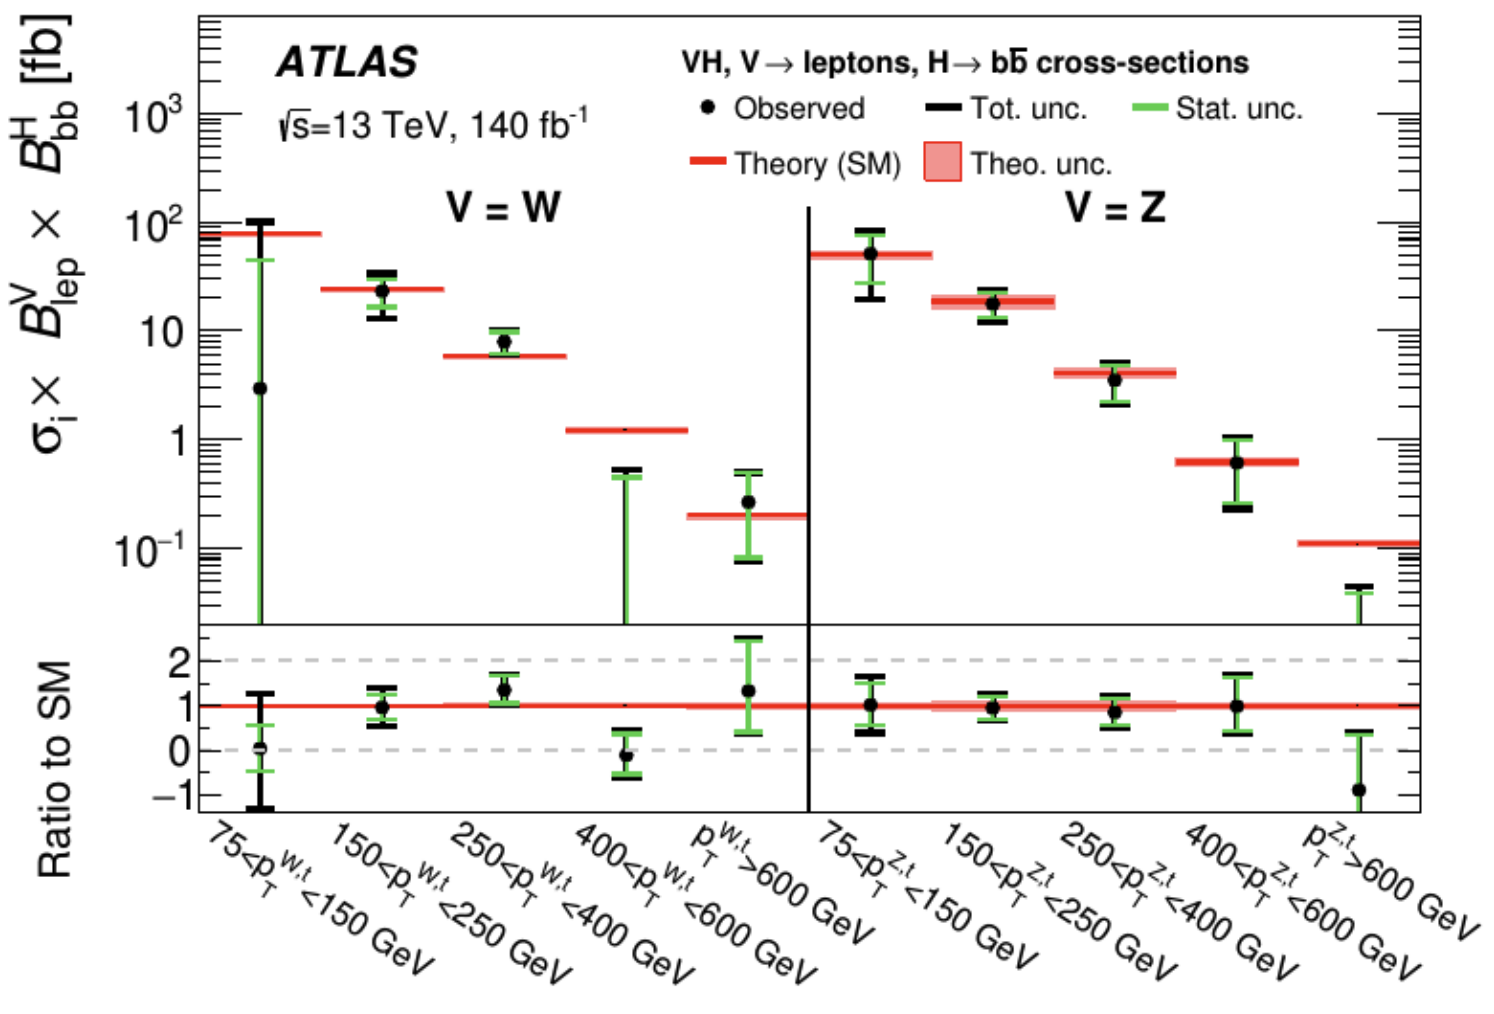
\includegraphics[width=0.45\textwidth]{figures/statistical/vhbb_differential_xsec.png}\label{fig:vh_bb_stxs_results_plot}
    }
    \caption{Comparison of the STXS differential cross-section measurements for (a) the $WH(WW^{*})$ channel from this analysis and (b) the $VH(b\bar{b})$ channel from the Run~2 analysis~\cite{ATLAS:2024yzu}. The $WH(WW^{*})$ results show much better sensitivity in the lower $\ptv$ bins, where the $VH(b\bar{b})$ analysis has limited or no sensitivity.}\label{fig:stxs_results_discussion}
\end{figure}

A comparison with the full Run~2 $VH(b\bar{b})$ analysis illustrates the complementary sensitivity of the \wh{} channel, particularly in the low-$\ptw$ regions. Figure~\ref{fig:stxs_results_discussion} compares the results of this analysis with those from the Run~2 $VH(b\bar{b})$ measurement~\cite{ATLAS:2024yzu}. The $VH(b\bar{b})$ analysis does not attempt to measure the lowest $\ptv$ bin due to overwhelming background contamination, resulting in negligible sensitivity. In addition, the $VH(b\bar{b})$ analysis exhibits limited sensitivity in the $75 \leq \ptv < 150$~GeV bin, where the measured signal strength is consistent with zero and associated with a large uncertainty. In contrast, the present analysis demonstrates meaningful sensitivity in both of the lower $\ptv$ bins, highlighting the importance of the \wh{} channel in probing regions of phase space that are inaccessible to other analyses. Likewise, the $VH(b\bar{b})$ channel provides superior sensitivity in the higher $\ptv$ bins, where the current analysis has almost no sensitivity.
